\begin{frame}{Unaprijedna umjetna neuronska mreža}
	\twocolumns{
\begin{figure}
	
	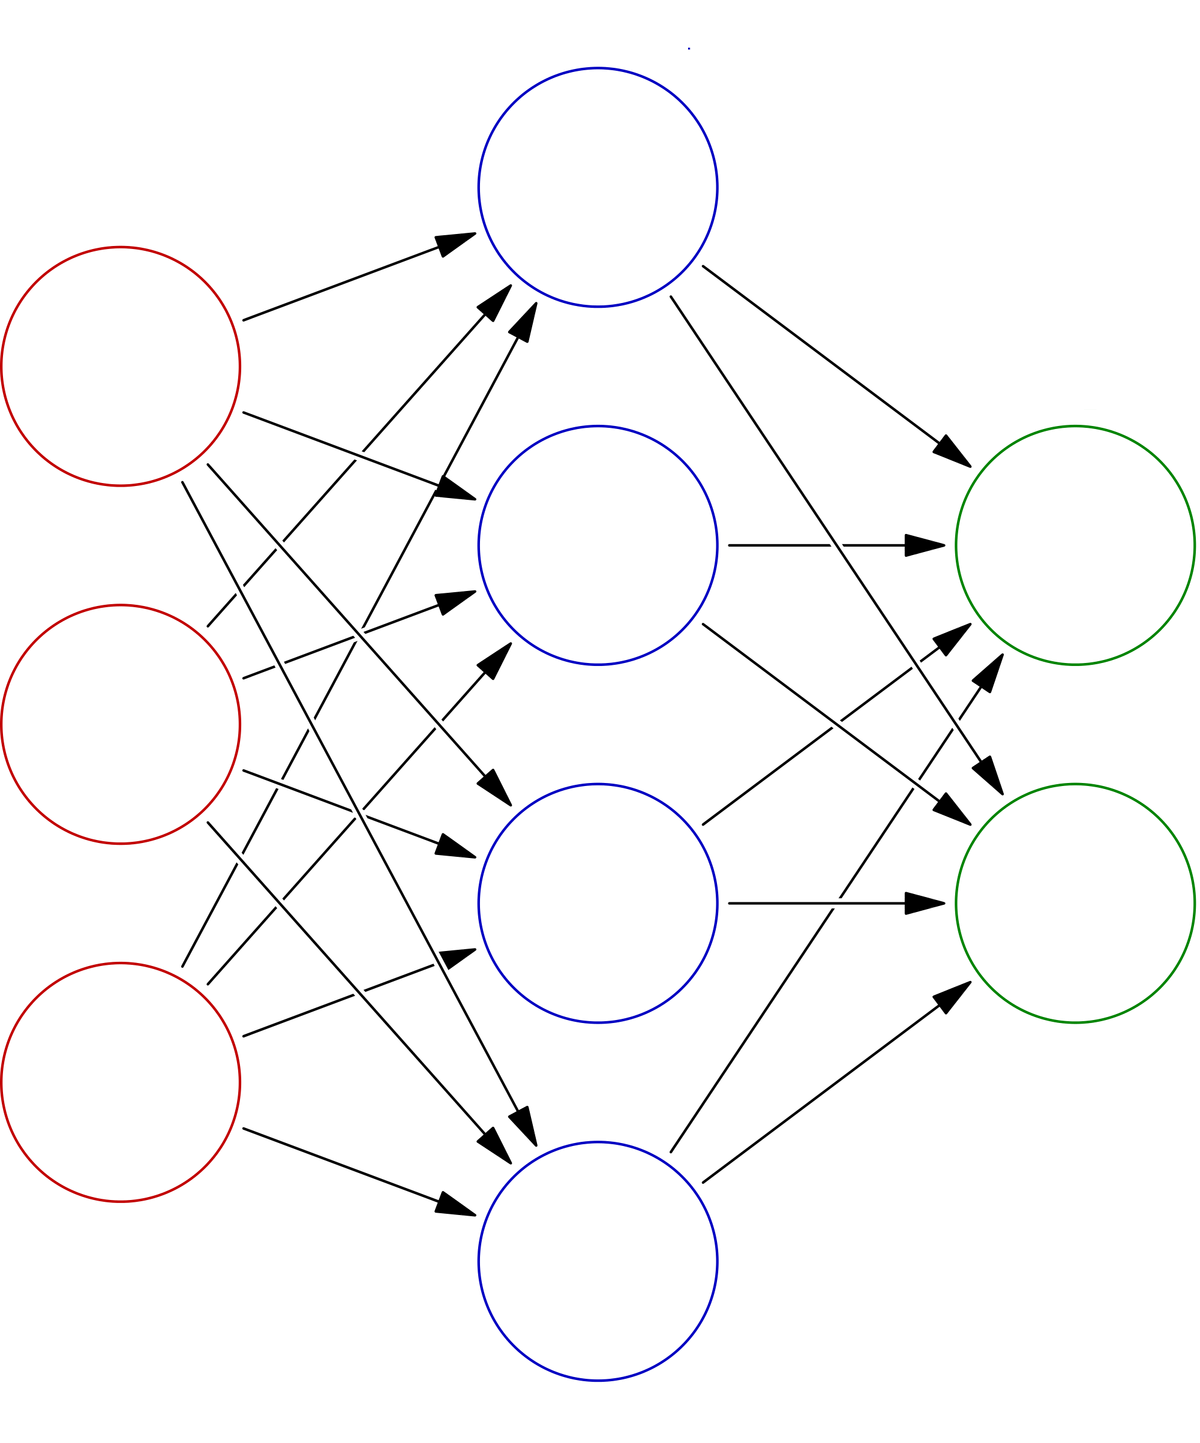
\includegraphics[width=1\textwidth]{slike/unaprijedna}
	\caption{Unaprijedna umjetna neuronska mreža \\ Izvor: automaticaddison, \textit{Artificial Feedforward Neural Network With Backpropagation From Scratch}}
\end{figure}
	}{
		\begin{itemize}
			\item \textbf{ulaz:} polje realnih brojeva iz igre dovodimo na ulazni sloj
			\item \textbf{izlaz:} igrač je odigrao akciju s najvećom vrijednosti u izlaznom sloju
			\item \textbf{u memoriji:} polje realnih brojeva (težine)
		\end{itemize}
	}
\end{frame}

\begin{frame}{Elmanova umjetna neuronska mreža}
	\twocolumns{
	\begin{figure}
	
	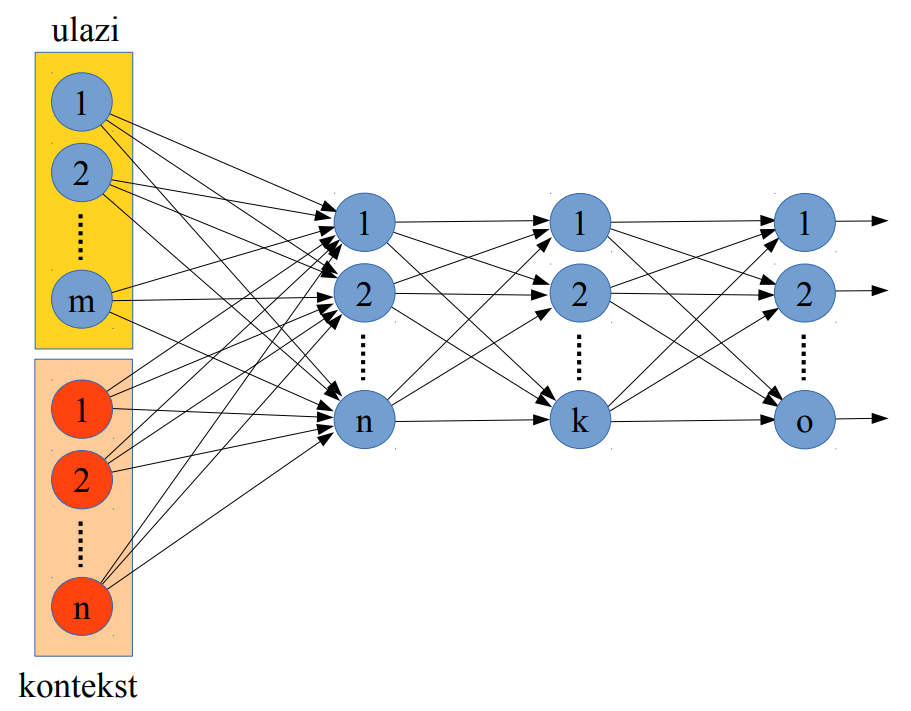
\includegraphics[width=1.25\textwidth]{slike/elman}
	\caption{Elmanova umjetna neuronska mreža \\ Izvor: Čupić, M. \textit{8. domaća zadaća – algoritam diferencijske evolucije}}
\end{figure}
}{
		\begin{itemize}
			\item \textbf{ulaz:} polje realnih brojeva iz igre dovodimo na ulazni sloj
			\item \textbf{izlaz:} igrač je odigrao akciju s najvećom vrijednosti u izlaznom sloju
			\item \textbf{u memoriji:} polje realnih brojeva (početne vrijednosti kontekstnog sloja i težine)
		\end{itemize}
	}
\end{frame}

\begin{frame}{Operatorsko stablo}
	\twocolumns{
\begin{figure}
\begin{forest}
for tree={
  l sep=30pt,
  parent anchor=south,
  align=center
}
[+
  [*,edge label={node[midway,left]{}}
    [-,edge label={node[midway,left]{}}
      [{[4]},edge label={node[midway,left]{}}
      ]
      [{[5]},edge label={node[midway,right]{}}
      ]
    ]
    [{[3]},edge label={node[midway,right]{}}
    ]
  ]
  [/,edge label={node[midway,right]{}}
	[{[3]},edge label={node[midway,left]{}}
    ]
    [{[5]},edge label={node[midway,right]{}}
    ]
  ]
]
\end{forest}
\caption{Operatorsko stablo za funkciju $([4] - [5]) \cdot [3] + [3] / [5]$}
\end{figure}
}{
		\begin{itemize}
			\item \textbf{ulaz:} polje realnih brojeva iz igre dovodimo na ulaz
			\item \textbf{izlaz:} igrač je odigrao akciju s indeksom $\floor{6 \cdot \frac{\sin{x} + 1}{2}}$
			\item \textbf{u memoriji:} stablo
		\end{itemize}
	}
\end{frame}

\begin{frame}{Programski isječak}
	\twocolumns{
\begin{figure}
\verbatiminput{test.lgp}
\caption{LGP program za izračun $R8 = (R4 - R5) \cdot R3 + R3 / R5$}
\end{figure}
}{
		\begin{itemize}
			\item \textbf{ulaz:} polje realnih brojeva iz igre ugradimo u registre
			\item \textbf{izlaz:} igrač je odigrao akciju s indeksom $\floor{6 \cdot \frac{\sin{\mathrm{R0}} + 1}{2}}$
			\item \textbf{u memoriji:} lista instrukcija
		\end{itemize}
	}
\end{frame}
